\documentclass[11pt]{article}  
\usepackage[margin=1in]{geometry}
\parindent=0in
\parskip=8pt
\usepackage{fancyhdr,amssymb,amsmath, graphicx, listings,float,subfig,enumerate,epstopdf,color,multirow,setspace,bm,textcomp}
\usepackage[usenames,dvipsnames]{xcolor}
\usepackage{hyperref}
\usepackage{graphicx}
\graphicspath{{./Images}}

\pagestyle{fancy}

\begin{document} 

\lhead{Assignment \# 8}
\chead{Robert Denim Horton}
\rhead{\today}

\begin{center}\begin{Large}
CS 4720 Networks, Crowds, and Markets

Homework \#  8

Student: (Robert Denim Horton)
\end{Large}
\end{center}

Suppose there are 2 ad slots each with its own clickthrough rate: 
\begin{center}
	\begin{tabular}{ |c|c|} 
		 \hline
		 Slot & Click Through Rate \\ 
		 \hline\hline
		 a & 10 \\ 
		 \hline
		 b & 7 \\ 
 		\hline
	\end{tabular}
\end{center}
And suppose there are 3 advertisers:
\begin{center}
	\begin{tabular}{ |c|c| } 
		 \hline
		 Advertiser & Valuation Per Click \\ 
		 \hline\hline
		 x & 10 \\
		 \hline 
		 y & 9 \\
		 \hline
		z & 2 \\ 
		 \hline
	\end{tabular}
\end{center}
We also suppose that the search engine assigns ad slots using a Gnereralized Second-Price (GSP) auction, and answer the following questions:

% Question 1
\begin{enumerate}
	 \item In this problem, is truthful bidding a Nash equilibrium? To receive full credit, you must either prove that truthful bidding is a Nash equilibrium or show which advertiser(s) could profit by changing their bid away from truthful bidding.
\end{enumerate}
% Question 1 Answers
\textcolor{gray}{
Answers:
\begin{enumerate}
	\item To begin solving this issue we can build a table to show whether or not truthful bidding would result in an N.E. This first table shows the different advertisers $x$, $y$,  and $z$.  Along the top row we have our different advertising slots $a$, $b$, and $c$. We add slot $c$ to add uniformity for this model and set its \textit{click-through-rate} to 0. Each slot has its own row with the corresponding revenue that the advertiser will get when winning the bid for that slot.  \\
	\begin{center}
		\begin{tabular}{ |c|c|c|c| } 
			\hline
			Advertisers & Slot a & Slot b & Slot c\\
			\hline \hline
			x & 100 & 70 & 0 \\
			\hline
			y & 90 & 63 & 0 \\
			\hline
			z & 20 & 14 & 0 \\ 
			\hline
		\end{tabular}
	\end{center}
We continue by building a table to show the results and tracks what the bidders value the slots at, what they are actually bidding, and the payoff from winning the slot they win. Now lets see if truthful bidding results in an N.E.
	\begin{center}
		\begin{tabular}{ |c|c|c|c|c|c| } 
			\hline
			Bidders & 	$v_j$ 	& 	$b_i$ 	& 	Slots 	& 	Prices 	&  Revenue - cost = payoff \\
			\hline \hline
			x 	  & 	10 	& 	10 	& 	a 	& 	9 	&  100 - 90 = 10\\
			\hline
			y 	  & 	9 	& 	9 	& 	b 	& 	2 	&  63 - 14 = 49 \\
			\hline
			z 	  & 	2 	& 	2 	& 	c	& 	0 	&  0 - 0 = 0 \\
			\hline
		\end{tabular}
	\end{center}
With the truthful table we see that bidder $y$ has a much higher pay off than $x$ and obviously $z$.  We can start a third table to keep track of the different payoffs corresponding to the amounts of each Advertiser's bid.
	\begin{center}
		\begin{tabular}{ |c|c|c|c|} 
			 \hline
			 Strategy & $x$ Payoff & $y$ Payoff & $z$ Payoff \\ 
			 \hline\hline
			 (10, 9, 2)\quad \textit{truthful} & 10 & 49 & 0 \\ 
	 		\hline
		\end{tabular}
	\end{center}
Now trying different values of bids we use the below values so that bidder $x$ now recieves slot $b$ and $y$ slot $a$.  So we get,
	\begin{center}
		\begin{tabular}{ |c|c|c|c|c|c| } 
			\hline
			Bidders & 	$v_j$ 	& 	$b_i$ 	& 	Slots 	& 	Prices 	&  Revenue - cost = payoff \\
			\hline \hline
			x 	  & 	10 	& 	8 	& 	b 	& 	8 	&  70 - 49 = 21\\
			\hline
			y 	  & 	9 	& 	9 	& 	a 	& 	2 	& 90 - 20 = 70 \\
			\hline
			z 	  & 	2 	& 	2 	& 	0	& 	0 	&  0 - 0 = 0 \\
			\hline
		\end{tabular}
	\end{center}
	\begin{center}
		\begin{tabular}{ |c|c|c|c|} 
			 \hline
			 Strategy & $x$ Payoff & $y$ Payoff & $z$ Payoff \\ 
			 \hline\hline
			 (10, 9, 2) \quad \textit{truthful} & 10 & 49 & 0\\ 
	 		\hline
			 (8, 9, 2) \quad \textit{untruthful} & 21 & 70 & 0\\ 
	 		\hline
		\end{tabular}
	\end{center}
	adding this to our table we see that the values for each bidder goes up and shows that truthful bidding would not yield a N.E.  
\end{enumerate}
}

% Question 2
\begin{enumerate}
	\setcounter{enumi}{1}
	\item  Find a Nash equilibrium for this problem (without truthful bidding) in which the total advertiser valuation is maximized (i.e., advertiser x is assigned slot a and advertiser y is assigned slot b). You may use any technique you want to find this Nash equilibrium, but you must convince me that it is an actual Nash equilibrium.
\end{enumerate}
% Question 2 Answers
\textcolor{gray}{
Answers:
\begin{enumerate}
	\setcounter{enumi}{1}
	\item Continuing from question 1 we can build off this and find the N.E. for this GSP using untruthful bids.  To do this we can simply try out different numbers for the bids, but something that was noticed is that the difference in-between the value of the bids of bidders $y$ and $z$ is very big and as we can see the difference between their payoffs is also very big. So, moving forward we construct another table where we show that the untruthful bids yield in a N.E. Using bid values 6, 3, and 0 for $x$, $y$, and $z$ respectively we get,\\
	\begin{center}
		\begin{tabular}{ |c|c|c|c|c|c| } 
			\hline
			Bidders & 	$v_j$ 	& 	$b_i$ 				& 	Slots 	& 	Prices 	&  Revenue - cost = payoff \\
			\hline \hline
			x 	  & 	10 	& 	 \textcolor{red}{6} 	& 	a	& 	 3	&  100\textcolor{red}{ - 30 = 70}\\
			\hline
			y 	  & 	9 	& 	 \textcolor{red}{3} 	& 	b 	& 	 0	&  63\textcolor{red}{- 0 =  63} \\
			\hline
			z 	  & 	2 	& 	 \textcolor{red}{0} 	& 	---	& 	--- 	&  \textcolor{red}{0} \\
			\hline
		\end{tabular}
	\end{center}
Which we see is a N.E. as bidder $x$ got worth greater than or equal to what slot $b$ would have yeileded (70), and bidder $y$ is happy as slot $a$ would have been to expensive.  Lastly $z$ cant really afford either one of these and thus N.E.
\end{enumerate}
}

% Question 3
\begin{enumerate}
	\setcounter{enumi}{2}
	\item Create a new sponsored search problem with at least 2 slots and at least 3 bidders in which truthful bidding is a Nash equilibrium.  We build the table to show the advertiser expected values associated with the clickthrough times the amount being payed for each click.
\end{enumerate}
% Question 3 Answers
\textcolor{gray}{
Answers:
\begin{enumerate}
	\setcounter{enumi}{2}
	\item Turns out, as discussed in class, we are able to use a " \textit{market clearing prices} " approach to yeild the N.E., we get the market clearing prices for the bidders as $MCP(41, 14, 0)$.  \\
	\begin{center}
		\begin{tabular}{ |c|c|} 
			 \hline
			 Slot & Click Through Rate \\ 
			 \hline\hline
			 a & 10 \\ 
			 \hline
			 b & 7 \\ 
	 		\hline
			 c & 0 \\ 
	 		\hline
		\end{tabular}
	\end{center}
	\begin{center}
		\begin{tabular}{ |c|c| } 
			 \hline
			 Advertiser & Valuation Per Click \\ 
			 \hline\hline
			 x & 10 \\
			 \hline 
			 y & 9 \\
			 \hline
			z & 2 \\ 
			 \hline
		\end{tabular}
	\end{center}
	\begin{center}
		\begin{tabular}{ |c|c|c|c| } 
			\hline
			Advertisers & Slot a & Slot b & Slot c\\
			\hline \hline
			x 	& 	100 \textcolor{red}{- 41 = 59} 	& 	70 \textcolor{red}{ - 14 = 56} 	& 0 \\  % 
			\hline
			y 	& 	90 \textcolor{red}{- 41 = 49} 	& 	63 \textcolor{red}{ - 14 = 49} 	& 0 \\  %
			\hline
			z 	& 	20 \textcolor{red}{- 41 = -21}	& 	14 \textcolor{red}{ - 14 = 0} 	& 0 \\  %
			\hline
		\end{tabular}
	\end{center}
	With this table we can construct a biparte graph with the advertisers and ad slots as show below
	\begin{center}
	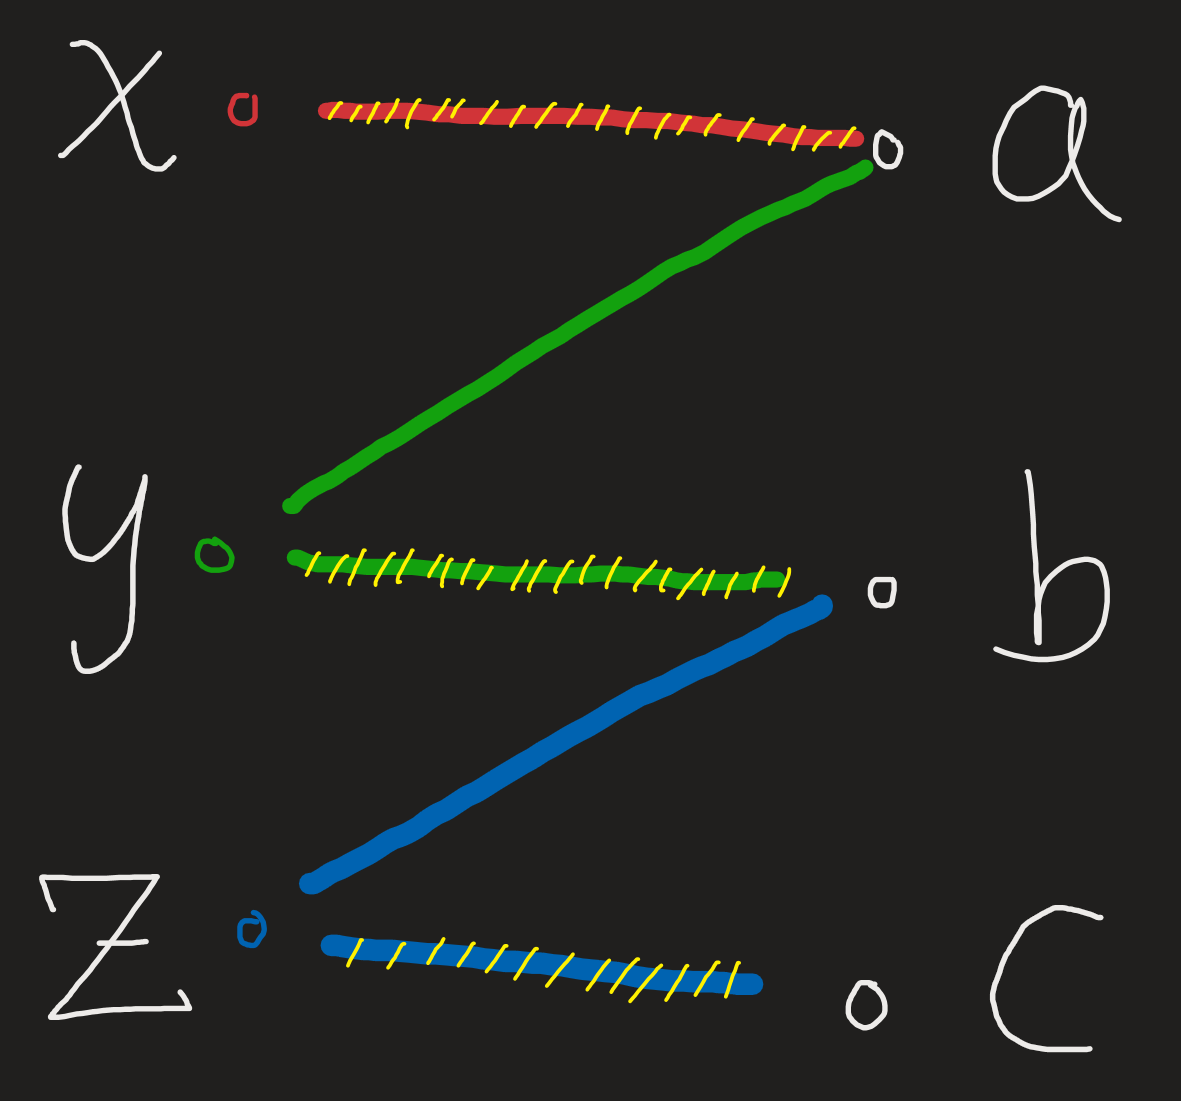
\includegraphics[scale=0.5]{Figure1.1}//
	\end{center}
	We can then see that each bidder has a preferred slot and now we can use these values to construct a GSP where truthful bids are a N.E.	So we can construct the graph below with the values we used 41, 14, and 0 being the optimal payoffs for bidders $x$, $y$, and $z$ respectively.  with these values we derive what they should bid into the table below.  We can then get the price per click by diving this be the respective valuation per slot.  so we get 41/10, 14/9, and 0 or \textit{price-per-click(4.1, 1.56, 0)}.
	\begin{center}
		\begin{tabular}{ |c|c|c|c|c|c| } 
			\hline
			Bidders & 	$v_j$ 	& 	$b_i$ 					& 	Slots 	& 	Prices 	&  Revenue - cost = payoff \\
			\hline \hline
			x 	  & 	5 	& 	 \textcolor{red}{$5$} 		& 	a	& 	4.1 	&  50 \textcolor{red}{ - 41 = 59}\\
			\hline
			y 	  & 	4.1 	& 	 \textcolor{red}{4.1} 		& 	b 	& 	1.56	& 63  \textcolor{red}{ - 10.92 = 52.08} \\
			\hline
			z 	  & 	1.56 	& 	 \textcolor{red}{1.56} 		& 	---	& 	--- 	&  0 \textcolor{red}{ - 0 = 0} \\
			\hline
		\end{tabular}
	\end{center}
	Thus, we have N.E. when bidder $x$ bids 5 and bidder $y$ bids 4.1.  Bidder $z$ does not want to bid anything as they can not afford to do so.  This process also gives us the \textit{socially}-optimal N.E. for this GSP as their will always be a N.E. in a GSP as given as a fact in class.
\end{enumerate}
}
\end{document}
